
\RequirePackage{fix-cm}

\documentclass[twocolumn]{svjour3}
%\flushbottom

\smartqed 

\usepackage{stfloats}
\usepackage{amsmath}
\usepackage{amsfonts}
\usepackage{amssymb}
\usepackage{xfrac}


%% Give the name of the journal


%% Give the author list to appear in the running head
%% Example \runauth{C.V. Radhakrishnan et al.}

%\biboptions{sort&compress}

% \biboptions{}

% if you have landscape tables
\usepackage[figuresright]{rotating}
\usepackage{subcaption}
\usepackage{booktabs}
% declarations for front matter

\usepackage[dvipsnames]{xcolor}
\usepackage{algorithm}
\usepackage{algpseudocode}
%\usepackage{subfig}
\usepackage{multirow}


\usepackage[shortlabels]{enumitem}
\setlist[enumerate]{nosep}

\usepackage{color}
\usepackage{soul}

\usepackage{setspace}

\usepackage{tabularx}
\newcolumntype{L}{>{\raggedright\arraybackslash}X}
\newcolumntype{Z}{>{\centering\let\newline\\\arraybackslash\hspace{0pt}}X}

\renewcommand{\vec}[1]{\mathbf{#1}}
\newcommand{\vv}[1]{``#1''}

\newcommand{\R}[1]{R#1}
\newcommand{\Ri}{\R{i}}
\newcommand{\RA}{\R{1}}
\newcommand{\RB}{\R{2}}

\newcommand{\qr}[1]{\mathbf{q}^{\R[1]}}
\newcommand{\qri}{\mathbf{q}^{\Ri}}
\newcommand{\qrA}{\mathbf{q}^{\RA}}
\newcommand{\qrB}{\mathbf{q}^{\RB}}

\newcommand{\qrik}{\qri_{k}}
\newcommand{\qqri}{\mathcal{Q}^{\Ri}}

\newcommand{\qrAk}{\qrA_{k}}
\newcommand{\qrAz}[1]{\qrA_{#1}}
\newcommand{\qrBz}[1]{\qrB_{#1}}
\newcommand{\qqrA}{\mathcal{Q}^{\RA}_{k}}

\newcommand{\qrBk}{\qrB_{k}}
\newcommand{\qqrB}{\mathcal{Q}^{\RB}}

\newcommand{\qris}{\qri_{s}}
\newcommand{\qrAs}{\qrA_{s}}
\newcommand{\qrBs}{\qrB_{s}}

\newcommand{\Tr}[2]{\mathbf{T}^{#2}_{#1}}
\newcommand{\Trk}[2]{\Tr{#1}{#2}|_k}

\newcommand{\ToolR}[2]{\Tr{#1}{ee_#2}}
\newcommand{\ToolRA}[1]{\ToolR{#1}{1}}
\newcommand{\ToolRB}[1]{\ToolR{#1}{2}}

\newcommand{\ToolRk}[2]{\Tr{#1}{ee_#2}|_k}
\newcommand{\ToolRAk}[1]{\ToolRk{#1}{1}}
\newcommand{\ToolRBk}[1]{\ToolRk{#1}{2}}

\newcommand{\wbigcup}[1]{\underset{#1}{\bigcup}}
\newcommand{\figref}[1]{Figure \ref{#1}} 


\definecolor{nero}{rgb}{0, 0,0}
\definecolor{rosso}{rgb}{0.9, 0,0}
\definecolor{verde}{rgb}{0, 0.6,0}
\definecolor{blu}{rgb}{0,0,0.9}
\definecolor{grigio}{rgb}{0.52,0.52,0.51}
\newcommand{\rev}[1]{\textcolor{verde}{#1}}
%\newcommand{\revout}[1]{\textcolor{rosso}{#1}}
\newcommand{\revout}[1]{}
%\newcommand{\revbar}[1]{\sout{#1}}
\newcommand{\revbar}[1]{}
\newcommand{\revgrey}[1]{\textcolor{grigio}{#1}}


\usepackage{afterpage}
\usepackage{longtable}

\usepackage[english=usenglishmax]{hyphsubst}
\usepackage{microtype}


\journalname{The International Journal of Advanced Manufacturing Technology}

\titlerunning{Int. J. of Adv. Man. Tech.}
\authorrunning{Stefano Mutti et al.}

\begin{document}
	
	\title{Optimal task positioning in multi-robot cells, using nested meta-heuristic swarm algorithms}
	
	
	\author{Stefano Mutti    \and
			Giorgio Nicola 	\and
			Manuel Beschi	\and
		    Nicola Pedrocchi \and
		    Lorenzo Molinari Tosatti
	}
	
	
	\institute{S. Mutti, N. Pedrocchi, L. Molinari Tosatti
	    \at Consiglio Nazionale delle Ricerche, Institute of Industrial Technologies and Automation, via A. Corti 12, Milan, Italy\\
		\email{stefano.mutti@stiima.cnr.it}           
        \and 
        G. Nicola \at Università di Padova, 
        Department of Information Engineering (DEI), via Gradenigo 6/A, Padua, Italy
        \and 
        M. Beschi \at Università di Brescia, Dipartimento di Ingegneria Meccanica ed Industriale, via Branze 38, Brescia, Italy
	}
	
	\date{Received: date / Accepted: date}
	% The correct dates will be entered by the editor
	
	\microtypesetup{activate=false}
	
  
  
    \maketitle
    
	\keywords{Multi-robot coordination; Motion planning;  optimization algorithms; industrial robotics;}

\begin{abstract}
While multi-robot cells are being used more often in industry, the problem of coordination of relative movements is still solved using heuristics and the human experience and,  in most cases, even a feasible solution takes a considerable amount of time to be found. Indeed, the optimization of generic performance index along the path, is complex due to the dimension of the feasible-configuration space. 
This work faces this challenge by proposing a layered-optimization method that integrates a Whale Optimization and an Ant Colony Optimization, and the method allows the minimization of user-defined functions to select the optimal solution in the feasible-configuration space.
\end{abstract}






\section{Introduction}
\label{introduction}


\begin{figure}[t]
	\centering
	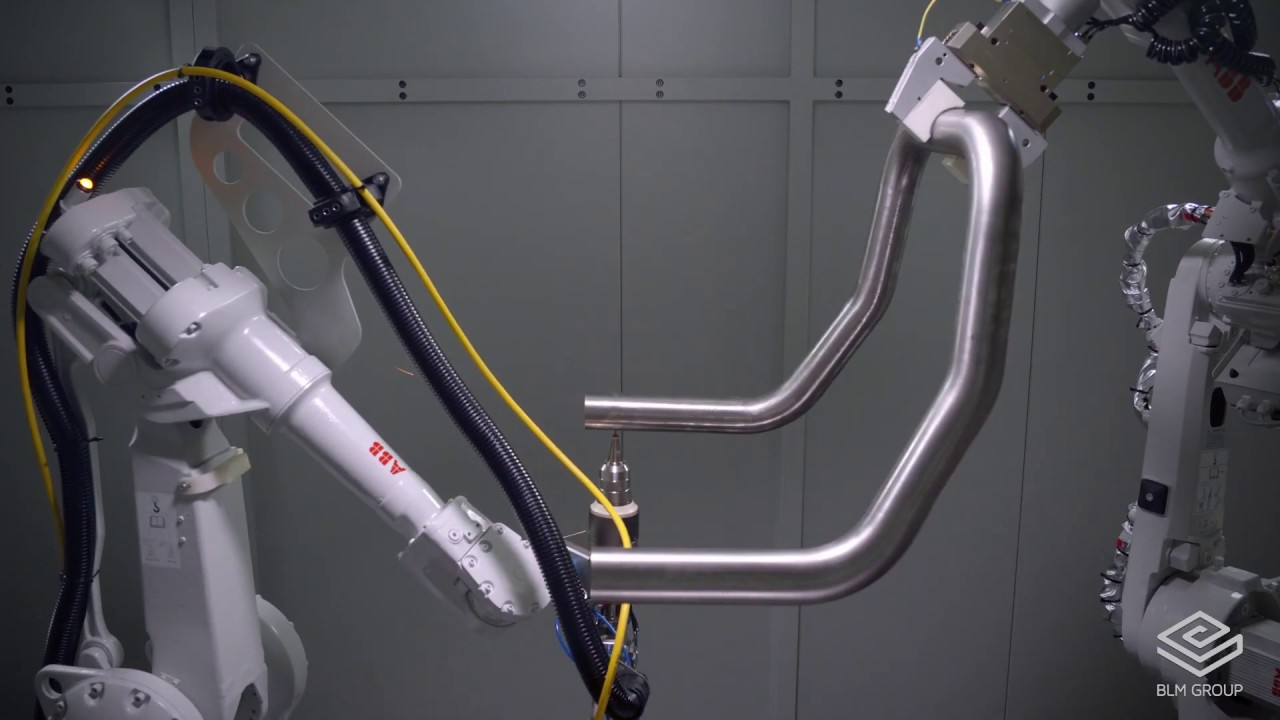
\includegraphics[trim={0 0.25cm 0 0.25cm},clip, width=0.8\columnwidth]{maxresdefault.jpg}
	\caption{Laser Cutting performed by two cooperative Robot (LT360 from BLM Group,  \cite{blmlt360})}
	\label{fig:blm}
\end{figure}

Working cells composed of multiple robots, as the one shown in \figref{fig:blm},  are being used more often for a huge variety of industrial tasks (\textit{e.g.}, welding, laser cutting, painting, \textit{etc.}) \cite{blmlt360,chen2013robot,ji2019industrial}, for their dexterity, reconfigurability.
In such a configuration, the position where the robot holds the work-piece strongly affects the operation feasibility (\textit{e.g.}, respect of the joints limits)  as well as the performance in term of path tracking as the direct consequence of the different robot kinematics (\textit{e.g.}, different joints speed, accelerations, friction, \textit{etc.}). 
%
The identification of a good position is a time consuming procedure even for skilled operators.
%
The operator, indeed, has to find collision free trajectories for the robots, that is far to be easy for many operation, especially when the tool has to be re-oriented. In such a case, according to the tool dimension, a small Cartesian movement of the tool center point (TCP) often forces the robot to span a large movement at the joint level\footnote{Consider \figref{fig:blm}. To contour a tube of 50mm the wrist center has to follow a circumference of about 1m as diameter}, and the identification of a configuration for which the operation is feasible is challenging due to the limited range of motion of many axes, and the likely collision between the links during the movement. 
%
Many off-the-shelves software tools (\textit{e.g.}, \cite{siemensPLMNX,abbRobotStudio}) allow the operator relaxing the constraints along the paths (see \figref{fig:task-redundacy}), and thanks to local gradient-based optimization they slightly modify the orientation of the tool to avoid collisions and to limit the joints motion as much as possible. 
However, these tools are not able to find solutions when the cell is complex or multi-robotic arm. 
%
\begin{figure}[t]
\centering
  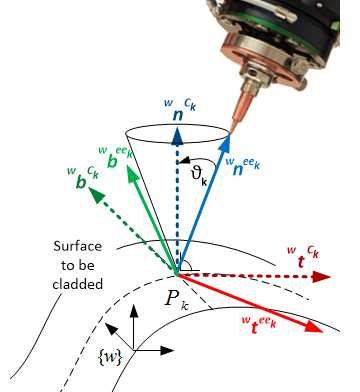
\includegraphics[trim={0 0.6cm 0 0.6cm},clip, width=.65\columnwidth]{TechnologicalRedundancy.png}
  \caption{Example of cladding application. The axis of the deposition head must lie in a cone centered with the surface normal direction, without quality deterioration.}
  \label{fig:task-redundacy}
\end{figure}
%
In literature, considering a single-arm workcell, this problem is generally tackled by the maximization of dexterity along the path~\cite{Yoshikawa1985,Angeles1992,siciliano2009,legnani2010,LACHNER2020103722}. However, such indexes do not consider problems such as backlashes or transmissions elasticity that cause poor robot accuracy even after static calibration. 

To overcome such limitations, many works~\cite{Feddema1996,Pamanes1991,Kamrani2008,Santos2010,Vosniakos2010} propose methods tailored on specific tasks and setup that may be extended to multi-arm workcells.
%
Specifically, in~\cite{Feddema1996}, the optimization is performed by a gradient method, that, however, may lead to the identification of a local minimum, without the possibility to span all the alternative robot configurations.  
Pamanes et al.~\cite{Pamanes1991} proposes a non-linear programming technique requiring at the beginning a candidate solution that satisfies all the constraints. The work relaxes the velocity constraints, \textit{i.e.}, the robot is supposed to be able to change configuration between two consecutive nodes, but the approach is not full-automatic and it is not suitable for when the problem is computationally complex.
%
Karamani et al.~\cite{Kamrani2008} proposes a response surface method but, since the objective function and the output are interpolated, the optimal solution might be very far from the global minimum due to the inaccuracy introduced by interpolation model adopted. Furthermore, they superimpose the robot configuration making bijective the inverse kinematics function. 
%
Santos et al.~\cite{Santos2010} proposes a tunneling method for searching the global minimum, but since the algorithm numerically solves a highly non linear equation many times, it is not suitable for all those application in which the computational time is as relevant. 
%
In~\cite{Vosniakos2010}, instead, the optimization is performed by two consecutive genetic algorithms, making complex the balancing between exploration and exploitation. 

As alternative to the path optimization, a few works \cite{tay1996optimising,son2019convex} address this problem focusing on the cell layout optimization, but despite the methods are interesting this practice is unlikely applicable in industry, where the robotic cell is used for many different operations.

%
Generally, optimization techniques are unsatisfactory for cooperative robotic tasks. First, the domain research space is huge, and the domain space may be a non-connected manifold since the constraints are always expressed in the Cartesian space but the inverse kinematics is not a bijective function. 
%
Also, even infinite solutions may be possible if the task is lazy-constrained (\textit{e.g.}, when the tool can rotate around its own axis). 
%
A tentative to cope with these issue is in \cite{Nicola2018}. The work focuses on the optimization of the workpiece positioning, taking in account only the kinematic redundancy of the robots involved. The methodology consists of splitting the problem in two sub-problems, and to run iteratively two nested optimizers: first the problem of the object positioning is solved (\textit{e.g.}, definition of the Robot-2 holding position), then, the Robot-1 redundant path is optimized. Finally, an iteration over the two steps is computed. This work, however, do not consider the technological redundancy (see \figref{fig:task-redundacy}), and the trajectory is fully constrained, \textit{i.e.}, the robot tool orientation must be properly aligned as the Frenet frame in each trajectory point. On the one hand, this assumption keeps limited the research space. On the other hand, it reduces dramatically the applicability of the methodology.
%
Among the plenty of optimization algorithms,  \cite{Nicola2018} proposes to use a Whale Optimization Algorithm (WOA) and an Ant Colony Optimization algorithm (ACO) for the first and second optimization steps respectively. On the one hand, Mirjalili et al.~\cite{Mirjalili2016} prove that WOA is among the best-performing meta-heuristic algorithms on a large set of mathematical problems. On the other hand, the ACO is extremely efficient when a combinatory problem has to be solved~\cite{Dorigo2006}. 


Starting from \cite{Nicola2018},  this work brings two major upgrades: it introduces a new method to
deal with the dimension of the search space allowing the integration in the model of the task redundancies, and it integrates an efficient collision checking strategy to remove from the research graph all the unfeasible trajectories. 
%
As remark, the collision checker ensures that the search of the best path in the redundant space avoids the exploration in proximity of unfeasible paths.

The paper is organized as following: in Section \ref{sec:problem} the optimization problem is mathematically formulated, in Section \ref{WACO} the optimization methodology is presented, highlighting the advancement with respect to \cite{Nicola2018}, in Section \ref{Perf_ana} the analysis of a paradigmatic use case is reported, and some general considerations on the methodology performance are discussed. . 


%The paper is organized as follow: in Section~\ref{WACO}, an iterative two-step optimization methodology to optimize the motion-coordinat\-ion of two robots is described; in Section~\ref{Perf_ana}, the analysis of the method performance is shown; finally, in Section~\ref{conclusions} conclusions and future developments are pointed out. 

\section{Problem Formulation}
\label{sec:problem}

Consider the generic robotic cell composed by a robot performing the desired task (Robot~1) and a robot holding the work-piece in static position (Robot~2) as shown in Fig~\ref{fig:robot_cell}. The affine transformation matrix $\Tr{R_1}{\RB}$ between the 2 robot base frames $\{\RA\}$ and $\{\RB\}$ is calibrated and known. For the $i$-th robot denote $\qri \in \mathbb{R}^{dof_i}$ as the vector of joint angles, with $dof_i$ is the joints number of the $i$-th robot, and $\Tr{\Ri}{ee^i}$ as the transformation from the base frame $\left\{\Ri\right\}$ to the end-effector frame $\{ee^i\}$ according to the forward kinematics, \textit{i.e.}, 
\begin{equation}
    \quad\Tr{\Ri}{ee^i}\equiv FK_{\Ri}\left(\qri\right)
\end{equation}
Regarding the inverse kinematics, denote $\qqri$ as the set of size $N_{sol}$ of the solutions in the considered pose, 
\begin{equation}
%\triangleq 
    \quad\qqri  \triangleq\left\{\qri_{1}, \ldots, \qri_{N_{sol}} \right\} = IK_{\Ri}\left(\Tr{\Ri}{ee^i}\right).
\end{equation}
As remark, the dimension $N_{sol}$ is a function of many factors: the kinematics of the robot, and the range of motion of the axes\footnote{if the axes are multi-turn, and/or if there are self-collision in some configurations}. 

Consider $\left\{0\right\}$ and $\left\{h\right\}$ the Absolute and the Work Object Frame respectively, where the Work Object Fra\-me is the frame that is used to describe the path that the robot has to follow to perform its own movement is defined. 
The path is a sequence of $N_{p}$ different nodes $\left\{p_k\right\}$, each described by a frame $\Tr{h}{p_k}$ with $k=1,\ldots, N_p$.\\
% \rev{definito pk}\\
The basic assumption that the Robot-2 is not moving while the Robot-1 performs the operation corresponds to impose that, at at the $k$-th trajectory node, the robots tool frame $\ToolRAk{0}$ and $\ToolRBk{0}$
\begin{subequations}\label{eq:problem}
\begin{align}
\quad\ToolRAk{0} & \equiv \Tr{0}{h}\,\Tr{h}{p_{k}}\label{eq:problem_r1},\\
\quad\ToolRBk{0} & \equiv \Tr{0}{h} \label{eq:problem_r2}.
\end{align}
\end{subequations}
%
\begin{figure}[t]
\centering
  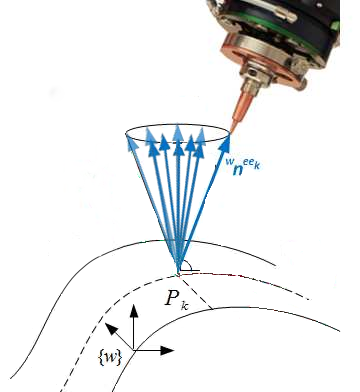
\includegraphics[trim={0 0.65cm 0 0.65cm},clip, width=.7\linewidth]{red_cone.png}
  \caption{Example of possible alternative configurations, exploiting the technological redundancy of the task.}
\end{figure}
%
\noindent The assumption in \eqref{eq:problem_r1} can be however relaxed for many nodes of the trajectory. Indeed, the robot tool pose often can differ from the Frenet frame assigned to the node, and technological redundancies can be exploited. Therefore, define $Alt\left( p_k \right)$ as the function that for each $\left\{p_k\right\}$  computes a set of possible alternatives satisfying given constraints (\textit{e.g.}, the tool lies inside a cone centred around the normal to the surface):
\begin{equation}\label{eq:redundancy_fcn}
    \quad
    A_k \triangleq \left\{\,\Tr{h}{a_{k,1}},\ldots,\,\,\Tr{h}{a_{k,N_{A}}}\,\,\right\} = Alt\left(p_k\right),
\end{equation}
where $N_{A}$ is a constant over $k$ denoting the dimension of the discretization of the searching space, and the first value of the set $A_k$ is equal to the nominal frame,
\begin{equation*}
\quad\Tr{h}{a_{k,1}}\triangleq \Tr{h}{p_k}
\end{equation*}
Once the set $A_k$ is computed for each $k$-th node of the trajectory, we can denote $C_k$ as the set of dimension $N_{C_k}$ of the feasible joint configurations $\qrA_1|_k$,  as
\begin{equation}
\begin{array}{lll}\label{eq:ck}
\quad C_k & \,\,\triangleq \,\, \left\{\qrA_1|_k,\ldots,\qrA_{N_{C_k}}|_k\right\}\\ \vspace{-6pt}\\
    &\,\,=\,\,\wbigcup{ s \leq N_{A_k}} 
%\qqrA \left( \Tr{\RA}{0}\Tr{0}{ee_2}\Tr{h}{p_k}\Tr{p_k}{a_{k,s}}\right)
\qqrA \left( \Tr{\RA}{0}\Tr{0}{h}\Tr{h}{a_{k,s}}\right)
\end{array}
\end{equation}
Worthily, the set $C_k$ is function of $\Tr{0}{ee_2}$, \textit{i.e.}, of the holding position as lead by Robot-2. 
However, in order to span only the configuration space of the Robot-1, it is possible to super-impose that the holding position is generated as starting position from Robot-1. 
Denote $\qrA_{start}$ as a starting joint configuration for the Robot 1, and $p_1$ as the first node of the trajectory. Closing the kinematics loop as show in Figure \ref{fig:robot_cell}, results in
\begin{equation}\label{eq:WACO_start_point}
\begin{array}{ll}
\quad \qqrB\,\,& \triangleq\,\,IK_{\RB}( \Tr{0}{h} )\,\,=\,\,IK_{\RB}( \Tr{\RB}{0}\,\Tr{0}{ee_1}\,\Tr{p_1}{h} ) \\ \vspace{-6pt} \\
    & =\,\,IK_{\RB}(\Tr{\RB}{\RA} \, FK_{\RA}\left(\qrA_{start}\right)\,\Tr{p_1}{h} ) 
\end{array}
\end{equation}
%
Once defined $\qrA_{start}$ is therefore possible to compute the search grid $\Gamma$ as 
\begin{equation}\label{eq:search-grid}
\quad    \Gamma\left(\qrA_{start}\right)\,\,\triangleq\,\,\left\{C_1, \ldots, C_{N_p}\right\} 
\end{equation}
The size of the research grid may be very large. As matter of example, consider a trajectory with 100 nodes. Assume that meanly for each node, 10 poses are feasible alternative poses, with a mean of 4 inverse-kinematics solutions each. Therefore, the number of possible trajectories are $ (4 \times 10)^{100}$  for each $\qrA_{start}$.

Finally, once the search grid is defined, it is mandatory to define a cost function to identify the best trajectories among the feasible ones.
The overall methodology has been called Whale and Ant Colony Optimization (WACO) and its pseudo code is shown in table Algorithm~\ref{alg_WACO}.
\section{Method}
\label{WACO}


\begin{algorithm*}[t!]
	\footnotesize
	\caption{WACO}
	\label{alg_WACO}
	\begin{algorithmic}[1]
		\State Load Task and robotic cell kinematic and geometric data
		\Function{WOA}{Kinematics}
		\While{$iter\leq$WOA max iterations}
    		\For{ each $i$-th whale }
    		    \State Initialize robots positions with $x_i$ hold value : $\qrA_{start} \leftarrow x_i$
        		\State Reconstruct Robot 1 kinematic : $\Tr{0}{h} \leftarrow \Tr{0}{h}(\qrA_{start})$
        		\State Calculate all path frames including the task redundancy :
        		\For{ $k <N_p$ }
        		    \State $\ToolRAk{0} \leftarrow \Tr{0}{h} \ToolRAk{h}$
        		    \State  $A_k \leftarrow Alt\left(\ToolRAk{0}\right)$
        		    \hspace{25em}\smash{$\left.\rule{0pt}{5.6 \baselineskip}\right\}\ \mbox{in parallel}$}
        		    \State Verify reachability and compute the possible IK solutions, $C_k \leftarrow f(A_k)$
        		\EndFor
        		\State Build the search graph : $\Gamma_i \leftarrow \qrA_{start}$
        		\State Assign all the weights to the feasible edges in the graph
        % 		\While{Collision free path is not found}
        % 		    \Function{ACO}{$\Gamma_i$}
        % 		    \State Calculate optimal $\RA$ path
        % 		    \hspace{15em}\smash{$\left.\rule{0pt}{1.0\baselineskip}\right\}\ \mbox{in parallel}$}
        % 		    \EndFunction~\Return Optimal $\RB$ configurations
        % 		    \State Collision check on best solution
        % 		    \If{path is not collision free}
        % 		        \State Update heuristics
        		        
    		  %      \EndIf
        % 		\EndWhile
        		\State ACO($\Gamma_i$) , see algorithm \ref{ACO}
        		\State Use ACO best solution to update the state of the WOA $x_i$
    		\EndFor
    		\State $iter \longleftarrow iter+1$
		\EndWhile
		\EndFunction~\Return{Optimal task position and robot joints}
	\end{algorithmic}
\end{algorithm*}

The here presented method is an improvement of \cite{Nicola2018}. Specifically, the contribution consists of the robust-stat\-istical discretization of the task-redundancy space, the integration of the collision detection and an improved ACO algorithm for graph optimization.

%Taking into account the task redundancy, it makes computationally complex the optimal-solution identification.
The algorithm is still composed of two nested iterative optimization methods.
The outside loop implements a Wha\-le Optimization Algorithm (WOA), an iterative meta-heu\-ris\-tic swarm optimization algorithm with a fixed number $N_{W}$ of particles called \vv{whales}. Each particle $x^n_i$,at every iteration $i$, takes as input the workcell geometry, the kinematic properties of the robots and the solution of the previous iteration, and it generates a new set of joint positions $\qrA_{start}|i $ for the Robot-1, and using the equation of the close kinematics of the two robots, the work object frame $\Tr{0}{h}|i$ can be therefore estimated.
%
This trajectory is a set of points, and for each points it is possible to super-impose a different set of constraints like the maximum misalignment between the tool axis and the surface normal direction, or the maximum Cartesian speed, \textit{etc.} according to the user needs.

\subsection{Research Space Discretization}

Halton sequences have been selected to discretize the task redundant space \cite{CHI20059}. The effectiveness of these sequences is related to the fact that they span homogeneously a research space, preserving the minimum distance between samples in a $k$-dimensional space \cite{Tijdeman75}. 
Specifically, consider an integer number $n$, and its representation in the base $b_j$ as
$$
n \equiv \sum_{i<M}a^{i}_{j,n} b_j^{i},
$$
with $M$ is an integer larger enough that all the digits of the number are represented, and each coefficient $a^i$ is $0 \leq a^{i}_{j,n} \leq b_j$.
The Halton sequence is constructed according to a deterministic method that uses coprime numbers as its bases, and following \cite{Kocis97}, we can compute a single Halton sequence as the $s$-tuple
$$
x_n = \left( \Phi_{b_0} (n),\ldots,\Phi_{b_s}( n) \right)
$$
where $\Phi_{b_j}(n)$ is the $j$-th radical inverse function:
$$
\Phi_{b_j}(n) = \sum_{i}a_{i}(j,n) b_j^{-i-1},
$$
To achieve the optimal covering of the space, a scramble of the coefficients is necessary, and the method in \cite{MATOUSEK1998527} has been implemented. 


% hence $Alt\left( p_k \right)$ is a function of the redundancy type parameterization , where the number of parameters depend on the geometric type of redundancy in use(e.g conic redundancy has 2 parameters, rotation redundancy has 1).

%\algrenewcommand\algorithmicindent{3.0em}%

%The WACO is intended to be computationally efficient, since each "whale" algorithms can run parallelly, and to reach an acceptable trade-off between the computation time and the solution accuracy. 

\begin{figure}[b]
	\centering
	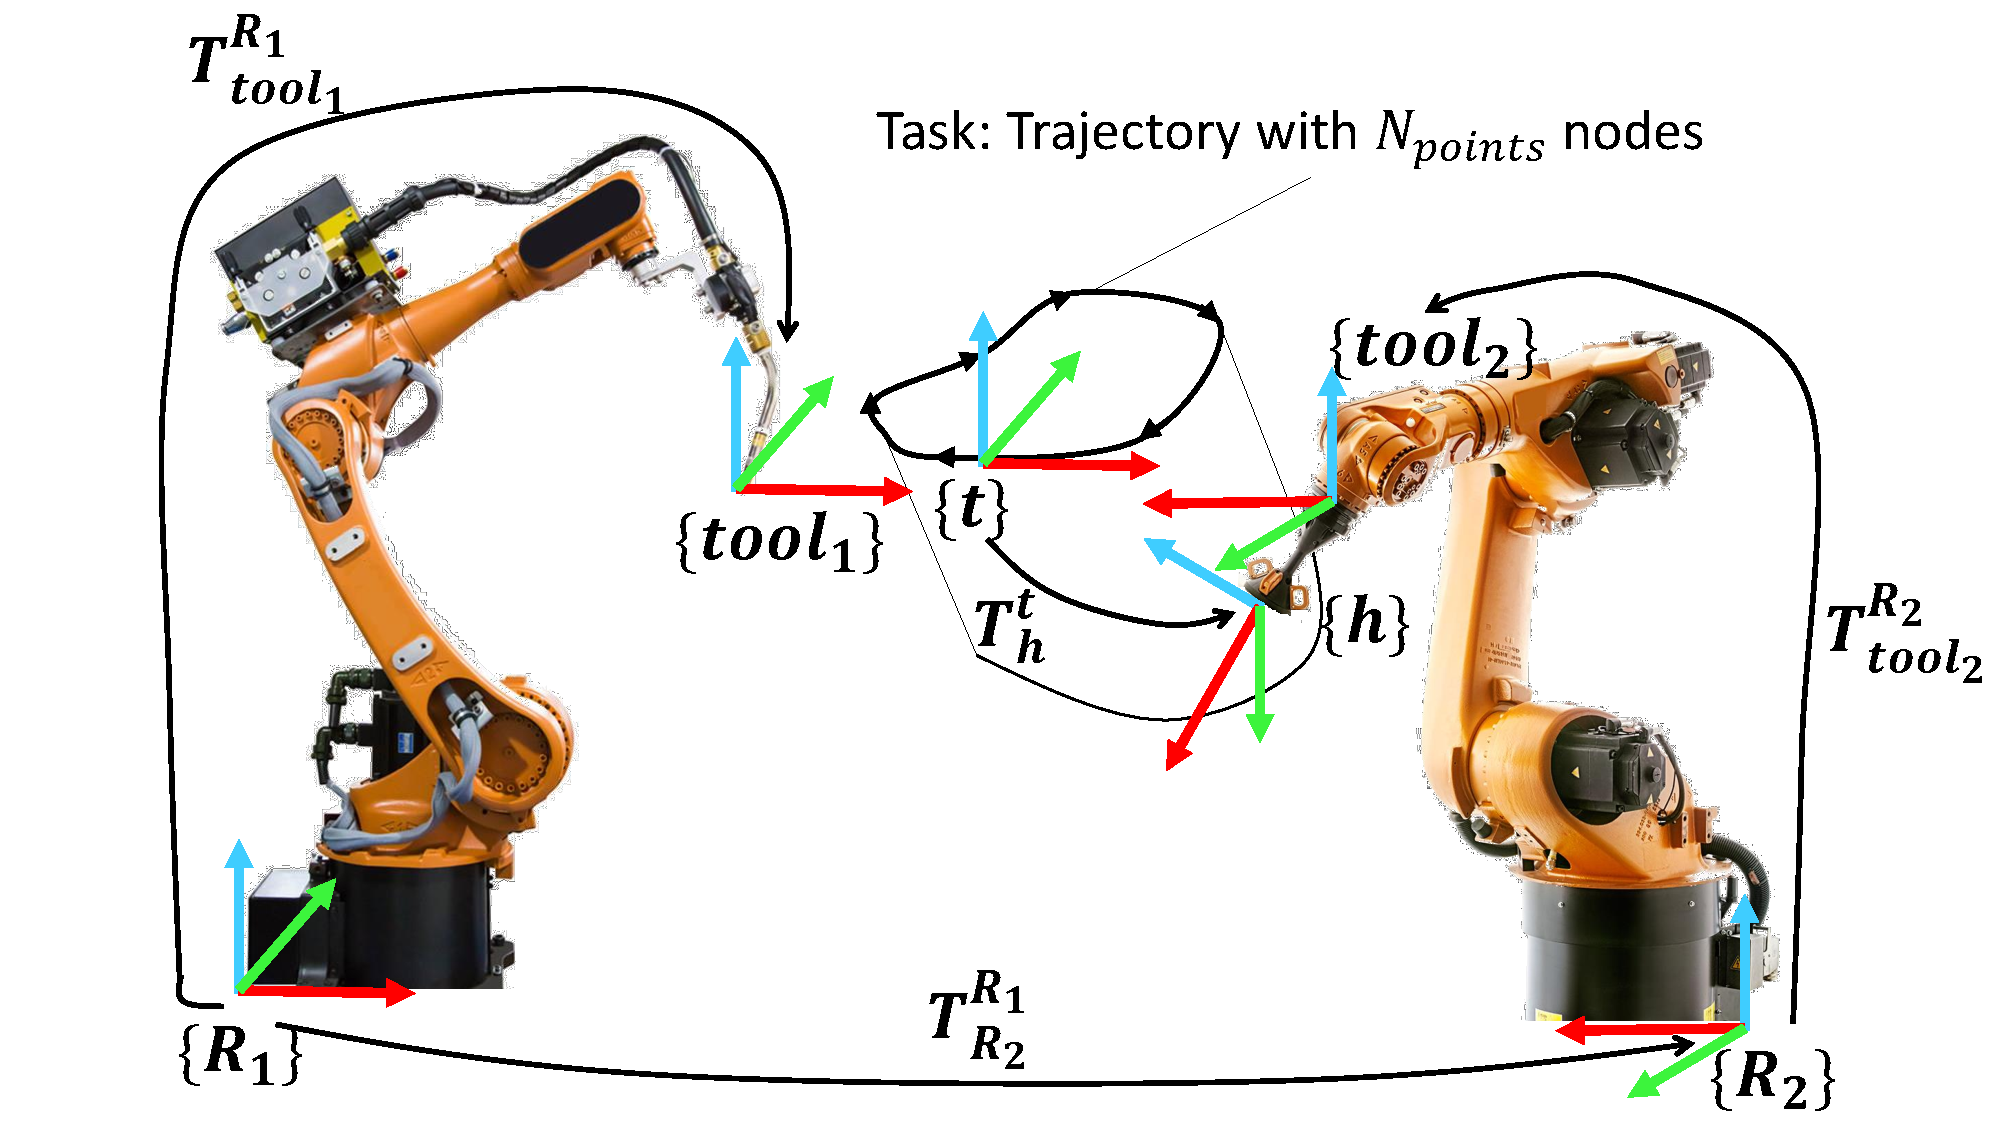
\includegraphics[width=0.99\columnwidth]{Robot_cell3}
	\caption{Robotic cell scheme}
	\label{fig:robot_cell}
\end{figure}
 
\subsection{First optimization layer: configuration calculus}
\label{WACO_optim}

Denote $i$ as the index counting the iteration of the WOA, and denote $x_n^i$ as the WOA particle that is properly initialized at each iteration.
Among the different possibility, we selected the Robot-1 joint positions as the WOA particle holded value, \textit{i.e.}, $x^i_0\equiv\qrAz{start}|i$.

Following the procedure described in Section \ref{sec:problem}, the search grid is therefore computed as \eqref{eq:search-grid}
$$
\quad    \Gamma_i \longleftarrow\Gamma  \left(\qrA_{start}|i\right)
$$
where the discretization of the research grid is performed using the Halton discretization as above described. 
Note that, if at least one path point with none valid configuration exists, the starting joint position is discarded. Specifically,
$$
\forall k \leq N_p \quad \quad C_k \neq \emptyset
$$
The search grid $\Gamma_i$ takes the form of a directed graph, where every node of the graph is a joint configuration, and each node associated to solutions in $C_{k=i} $ is connected to nodes of the following set $C_{k=i+1}$ (see  \figref{graph}), if the connection is a joint movement that satisfies the kinematic requirements.
Therefore, denote 
\begin{equation}\label{eq:graph-woa}
\quad\begin{array}{l}
\mathcal{P}_{i} =\left\{\qrA_{s_1}|_1,\ldots, \qrA_{s_k}|_k, \ldots, \qrA_{s_{Np}}|_{N_p}\right\}, \\ \vspace{-6pt}\\
\mbox{with} \quad \forall k \leq N_{p} \quad\quad \qrA_{s_k}|_k \in C_k 
\end{array}
\end{equation}
as the a feasible path from the starting pose to the final pose of the trajectory. 
In order to select the optimal $\mathcal{P}_{i}^*$ for each $i$-th WACO iteration, the ACO is used, and the method is described in Section \ref{sec_second_layer_ACO}. Once the $\mathcal{P}_{i}^*$ is computed, the evolution of the WAO is obtained by the evaluation of the underlying ACO resulted cost function, and the generation of a new set of robot joints value $\mathbf{q}^{\RA}_{start}|i+1$

\subsection{Second optimization layer: the path selection}
\label{sec_second_layer_ACO}

Ant Colony Optimization (ACO) is considered as the most performing algorithms for solving optimization problems~\cite{Dorigo2006}, and specifically for graphs as in \eqref{eq:graph-woa}.
%For each graph generated from the previous step, ACO is therefore used to compute the best trajectory, that is then outputted as result of the iteration.

%The optimization function has been chosen in order to minimize kinematic parameters related to the robot performing the task, such as joints speeds, accelerations and many more, or can be tailored to exploit path motion and position criterions that affect the final result for a specific task.
% \rev{cost func generale? spiegare negli experiments}
While the graphs to solve in \cite{Nicola2018} were almost trivial, the graphs in  \eqref{eq:graph-woa} have a considerable dimension, that depends on the discretization parameters.
For this reason, and through experimental analysis, the ACO algorithm in \cite{Nicola2018} have been revisited to cope with the new graph dimensions.
Specifically, we relied on a version called Elitist Max-Mix ACO, in which the pheromone deposited on a single node has a minimum and a maximum threshold, and the only solution taken in account at every iteration is the one with the highest objective function value.
The tuning of the algorithm's parameters follows \cite{pellegrini2006cal}, where the average of the solutions number per points  has been used as the number of nodes, instead that the whole number of nodes, due to the fact that our graph is not completely connected.


\begin{figure}[t]
	\centering
	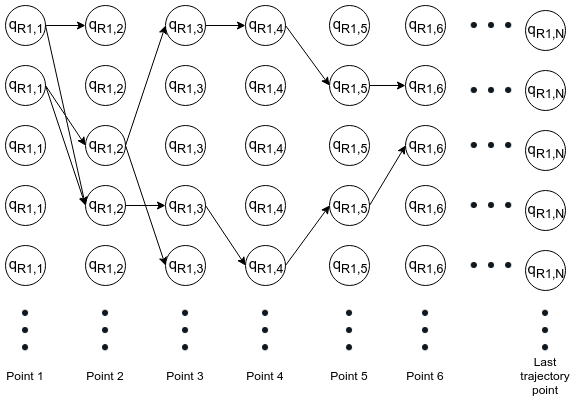
\includegraphics[height=5 cm]{graph}
	\caption{Simplified graph example.
	The columns hold different joint configurations for the trajectory points }
	\label{graph}
\end{figure}

Before feeding the graph to the optimization algorithm, all the weights of the connections between the nodes have to be properly set.
A node does not have a connection with a consecutive node, if the movement between the two is not possible due to kinematic constraints.
If the movement between two nodes satisfies the kinematic constraints, a strictly positive value is assigned to the edge connecting the two nodes.
The weights are called heuristic values, and will help the optimization algorithm "navigate" through the graph, especially in cases in which the graph dimension is considerable.
A commonly used heuristic is the joint distance between two consecutive points solutions:
\begin{equation}
\label{eq_ACO_heu}
heuristic=\frac{1}{\left(q^{R_1}_{k}-q^{R_1}_{k-1}\right)\left(q^{R_1}_{k}-q^{R_1}_{k-1}\right)}
\end{equation}
but many more can be used on the optimization criteria.
Once the graph is obtained, the ACO algorithm can be used to find a solution, refer to \cite{Dorigo2006} for an ACO survey.

The collision check has been designed in order to reduce the dimension of the graph used by the ACO. Indeed, as described in the section below, the collision checking purge from the graph all the configuration that are in collision, discarding solutions that are not feasible rather than including them in the optimization, for details see section \ref{coll}.

In algorithm \ref{ACO} is shown a simplified algorithm description.
Once the number of iterations has been reach\-ed, the best path found in all the iterations is given as output and used by the WOA for its next iteration.

\algrenewcommand\algorithmicindent{3.0em}%
\begin{algorithm*}[ht]
	\footnotesize
	\caption{ACO}
	\label{ACO}
	\begin{algorithmic}[1]
		\State Load $\Gamma_i$ for every particle in WAO
		\Function{ACO}{$\Gamma_i$}
		\While{$\mathcal{P}^*$ is not collison free}
		\While{$iter\leq$ACO max iterations}
		\State Calculate a path $\mathcal{P}_{i}$ on $\Gamma_i$ an in \eqref{eq:graph-woa}
		\hspace{15em}\smash{$\left.\rule{0pt}{2.0\baselineskip}\right\}\ \mbox{in parallel}$}
		\State Update pheromone value on the graph $\Gamma_i$ 
		\State $iter=iter+1$
		\EndWhile
		\State Select best solution among all graphs $\mathcal{P}^* = max(\mathcal{P}_{i})$
 		\If{ Check for collisions over $\mathcal{P}^*$, see algorithm \ref{alg_coll_det} }
		    \State return $\mathcal{P}^*$
		\Else
		    \State modify $\Gamma_i$ according to algorithm \ref{alg_coll_det}
		    \State iter = 0
        \EndIf
		\EndWhile
		\EndFunction~\Return{Optimal path found}
	\end{algorithmic}
\end{algorithm*}

\subsection{Collision Detection}
\label{coll}
Collision detection is computally demanding, and the number of possible combinations of robot cell joint position to be checked at every WOA iteration is equal to $N_{whales}\times \dim(\Gamma)$. Also, it increases exponentially with the number of discrete redundant configurations and points in the trajectory. In this module the collision detection problem was solved by using the state of art of collision detection libraries and by exploiting the peculiarities the problem studied. The collision detection is performed with the library GPU-Voxels~\cite{Hermann2014} that implements voxel based algorithms and that takes advantage of parallel computation on GPU to increase computational speed.\\
The first goal was to minimize the number of trajectory where to perform the collision detection, so it was decided to evaluate, among the $N_{whales}$ trajectories, only the one with the highest objective function  value defined previously as $\mathcal{P}^*_i$. Indeed, if $\mathcal{P}^*_i$ is collision free then it is not necessary to check the other trajectories, otherwise if $\mathcal{P}^*_i$ is not collision free performing the collision detection on the other trajectories and taking the best one collision free would not guarantee to be a better trajectory than collision-free solution of the graph $\mathcal{P}^*_i$ belongs. Then if $\mathcal{P}^*_i$ is not collision free and if the graph $\Gamma_i$ is still feasible, as it will be detailed later, a new solution to $\Gamma_i$ is computed and the collision detection will be performed on the new $\mathcal{P}^*_i$ that might belong to another graph. Otherwise if $\mathcal{P}^*_i$ is no longer feasible the collision detection will be performed on the trajectory with the highest objective value function among the remaining. This loop is performed till a collision free path is found or all the graphs are considered unfeasible.\\
The collision detection is divided in 3 parts in order to take advantage of the peculiarities of the involved problem,  collisions in the multi-robot cell studied can have various sources (robot - environment, robot- robot, tool - work-piece). Furthermore, since voxel based methods are used, the different collision sources require different level of discretization, for example the collision between the robots and the environment can be studied with a coarse discretization meanwhile, collisions between the tool and the workpiece since they are very close (e.g. in laser cutting the distance between the tool-head and the workpiece is generally less than 3~mm) a very high level of discretization is required. 
It can be easily noticed that once a collision is found in a graph node (i.e. trajectory points) based on the source it is possible to delete other nodes or even setting all the graph as unfeasible. In particular, a collision between the Robot2 and the environment since both are static set the entire graph as unfeasible, meanwhile a collision between the tool and the workpiece automatically deletes from the graph a number of nodes equal to the inverse kinematic solution for that specific position and orientation of the tool-head. So 4 different collision detection steps are performed with 2 different level of discretization.
\begin{enumerate}
	\item Robot2 - Environment (low discretization)
	\item Tool - Workpiece (high discretization)
	\item Robot1 - Environment (low discretization)
	\item Robot1 - Robot2 (low discretization)
\end{enumerate}
Finally, if a collision is found, except for the case of a collision between Robot2 and Environment, all the graph nodes belonging to the same trajectory point are checked before computing a new ACO solution so, the new solution is forced to pass by a set of collision free nodes highly reducing the search space for the solution. If no collision free node is found the graph is set as unfeasible. The pseudo-code is shown in Algorithm~\ref{alg_coll_det}. The order of the collision detection steps has been chosen to perform firstly the steps that can reduce the graph dimension more quickly.

\begin{algorithm}[t]
	\footnotesize
	\caption{Collision detection}
	\label{alg_coll_det}
	\begin{algorithmic}[1]
	\If {$Collision(Robot2, Env.)$}
	    \State \Return $\Gamma$ unfeasible
    \EndIf
	\For{each path point}
		\If{$Collision(Tool, Work.)$}
		    \For{ each tool orientation}
		        \If{$Collision(Tool, Work.)$}
		            \State Purge node
	            \EndIf
		    \EndFor
		    \State \Return
	    \EndIf
    \EndFor
    \For{each path point}
		\If{$Collision(Robot1, Env.)$}
		    \For{each Robot configuration}
		        \If{$Collision(Robot, Env.)$}
		            \State Purge node
	            \EndIf
	        \EndFor
	        \State \Return
	    \EndIf
    \EndFor
    \For{each path point}
		\If{$Collision(Robot1, Robot2)$}
		    \For{each Robot configuration}
		        \If{$Collision(Robot1, Robot2)$}
		            \State Purge node
	            \EndIf
	        \EndFor
	        \State \Return
	    \EndIf
    \EndFor
    \State \Return $\mathcal{P}^*_i$ collision free
	\end{algorithmic}
\end{algorithm}

\section{Performance Analysis}
\label{Perf_ana}

\subsection{Experimental setup}
\label{exp_setup}


The setup is composed by two ABB~IRB4600 20.5 (see \figref{fig:robot_cell} ) and it is configured for cooperative laser cutting application of industrial pipes.\\
% \rev{Figura 4 lontana?}
Different paths with varying number of points of have been tested and optimized by the algorithm, from simple circular holes and pegs on the pipes side, to a complete trimming of the tips.
The trimming of the tips, is considered to be a difficult operation due to the circular path of the robot around the pipe, the constraint of perpendicularity between the cutting head and the pipe surface and the collision possibility during the path execution.
For the simulation, the algorithm have been used in order to minimize the quadratic sum of the joints speed of the Robot 1,while keeping a safe distance from the joint limits, using a tailored objective function.
The algorithm have been tested with different parameters setup, specifically: 
For the whale optimization algorithm:
\begin{enumerate}[-]
	\item WOA iterations number
	\item Whales number
	\item WOA \vv{optimization/exploration} $A_{lim}$ parameter
\end{enumerate}
while for the ant colony optimization:
\begin{enumerate}[-]
	\item ACO iterations number
	\item Ant number 
	\item heuristic weight exponent value
\end{enumerate}
Different redundancies have also been tested, from the freely rotation around the cutting head $Z$ axis, to a more relaxed conic redundancy in which the head $Z$ axis can freely move inside a given cone with a small aperture.
The software designed to perform the tests, takes advantage of the ROS framework in order to import robot parameters from the ROS industrial \cite{rosI:2013} project repository, it also makes use of a modified version of the ikfast openrave library for computing the inversion kinematic of a robots in a parallel way on the GPU.
The simulations have been made on a desktop computer equipped with a NVIDIA GeForce gtx 1060 GPU, on which the algorithm has been designed, taking advantage of the CUDA libraries for parallel computation.
Due to the size of the memory needed for running the algorithm, which raises exponentially with the discretization parameters and trajectory points number, the tests performed have a limited number of parameters combination.
However, as shown by the collected results, the problem can be adequately solved with a limited amount of resources.  
\rev{github IRAS codice }



\subsection{Sampled results considerations}
All the simulations gave a feasible , collision free path as output.
In figures \ref{fig:sfig1},\ref{fig:sfig2},\ref{fig:sfig3}, are shown some significant results extracted from algorithms run on the same task with different WOA parameters.
The dotted lines show the best so far value of the objective function among all the WOA particles at every iteration, while the dashed line shows the average of the dotted lines.
The continuous lines show the average value of the objective function hold by all the whales particles at every iteration.
All the performed simulations, regardless of the parameters value, have shown a predictable trend, in which it is noticeable the presence of 2 distinct phases.
During the first phase, the whales particles "explore" the joint space of the robots, the hold solutions are diverse(as shown by the difference between the average value, continuous lines, and the best so far values, dotted lines) and constantly change due to the WAO algorithm nature and its parameters value.
In the second phase the solution are refined, the WOA algorithm particles move in proximity of their solutions and the exploration is concluded, the search is now focusing on optimizing the best solutions found, settling on the nearest optimum points.
The simulations are repeated 5 times for each parameters combination in order to have a statistical sample.



\begin{figure}[h]
    	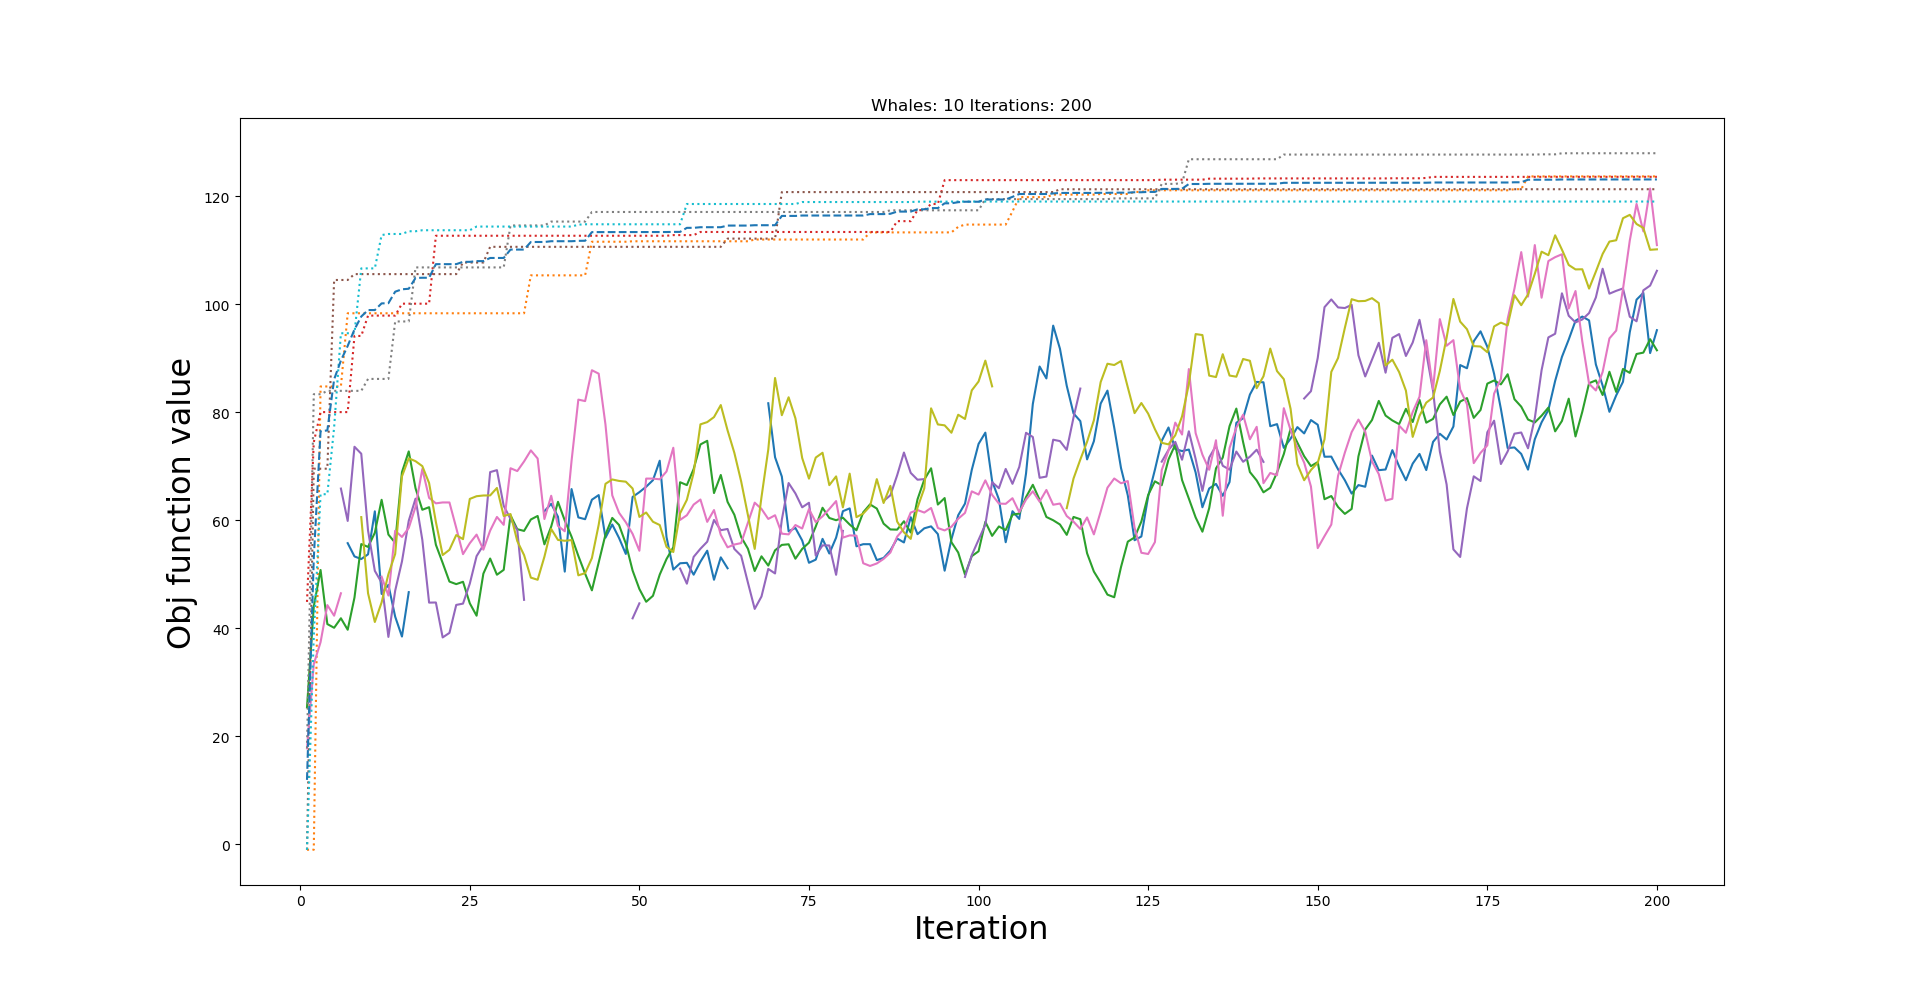
\includegraphics[width=1\linewidth]{Figure_6}
        \caption{Objective function trends for peg hole task with 10 whales particles for 200 iterations}\label{fig:sfig1}
\end{figure}
\begin{figure}[h]
		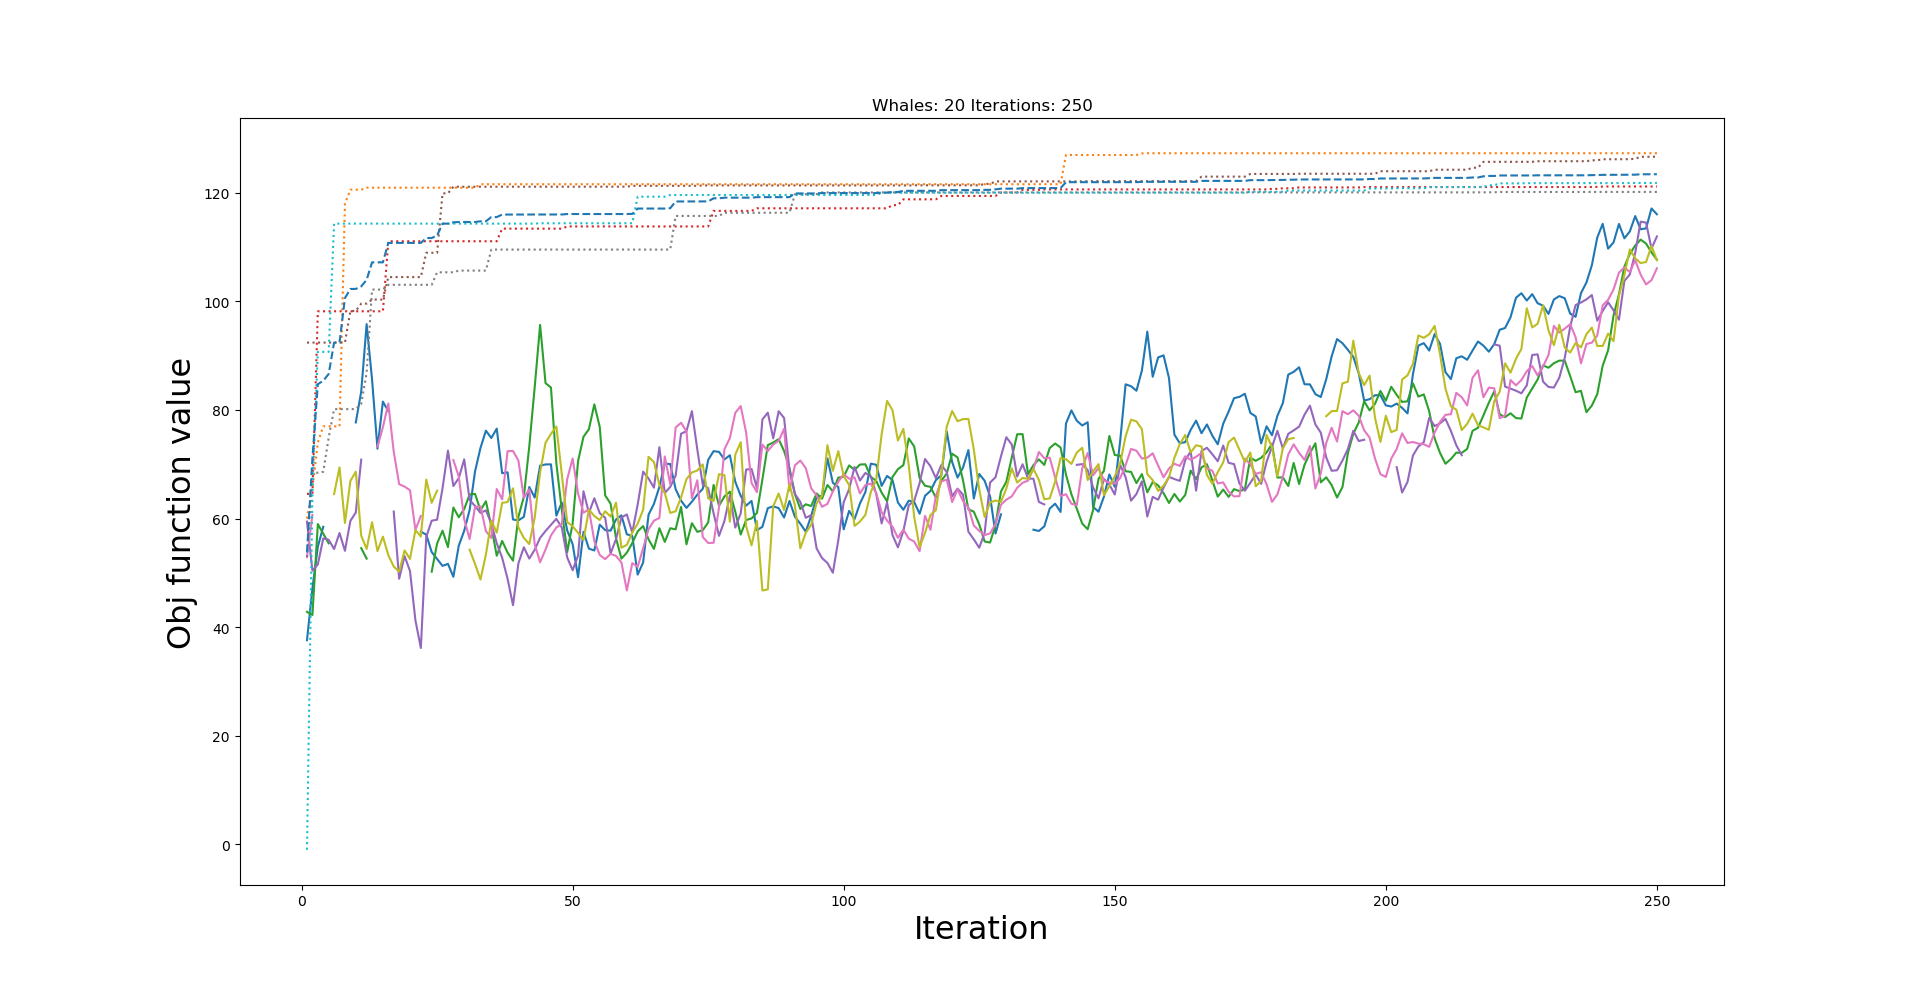
\includegraphics[width=1\linewidth]{Figure_5}
        \caption{Objective function trends for peg hole task with 20 whales particles for 250 iterations}\label{fig:sfig2}
\end{figure}
\begin{figure}[h]
		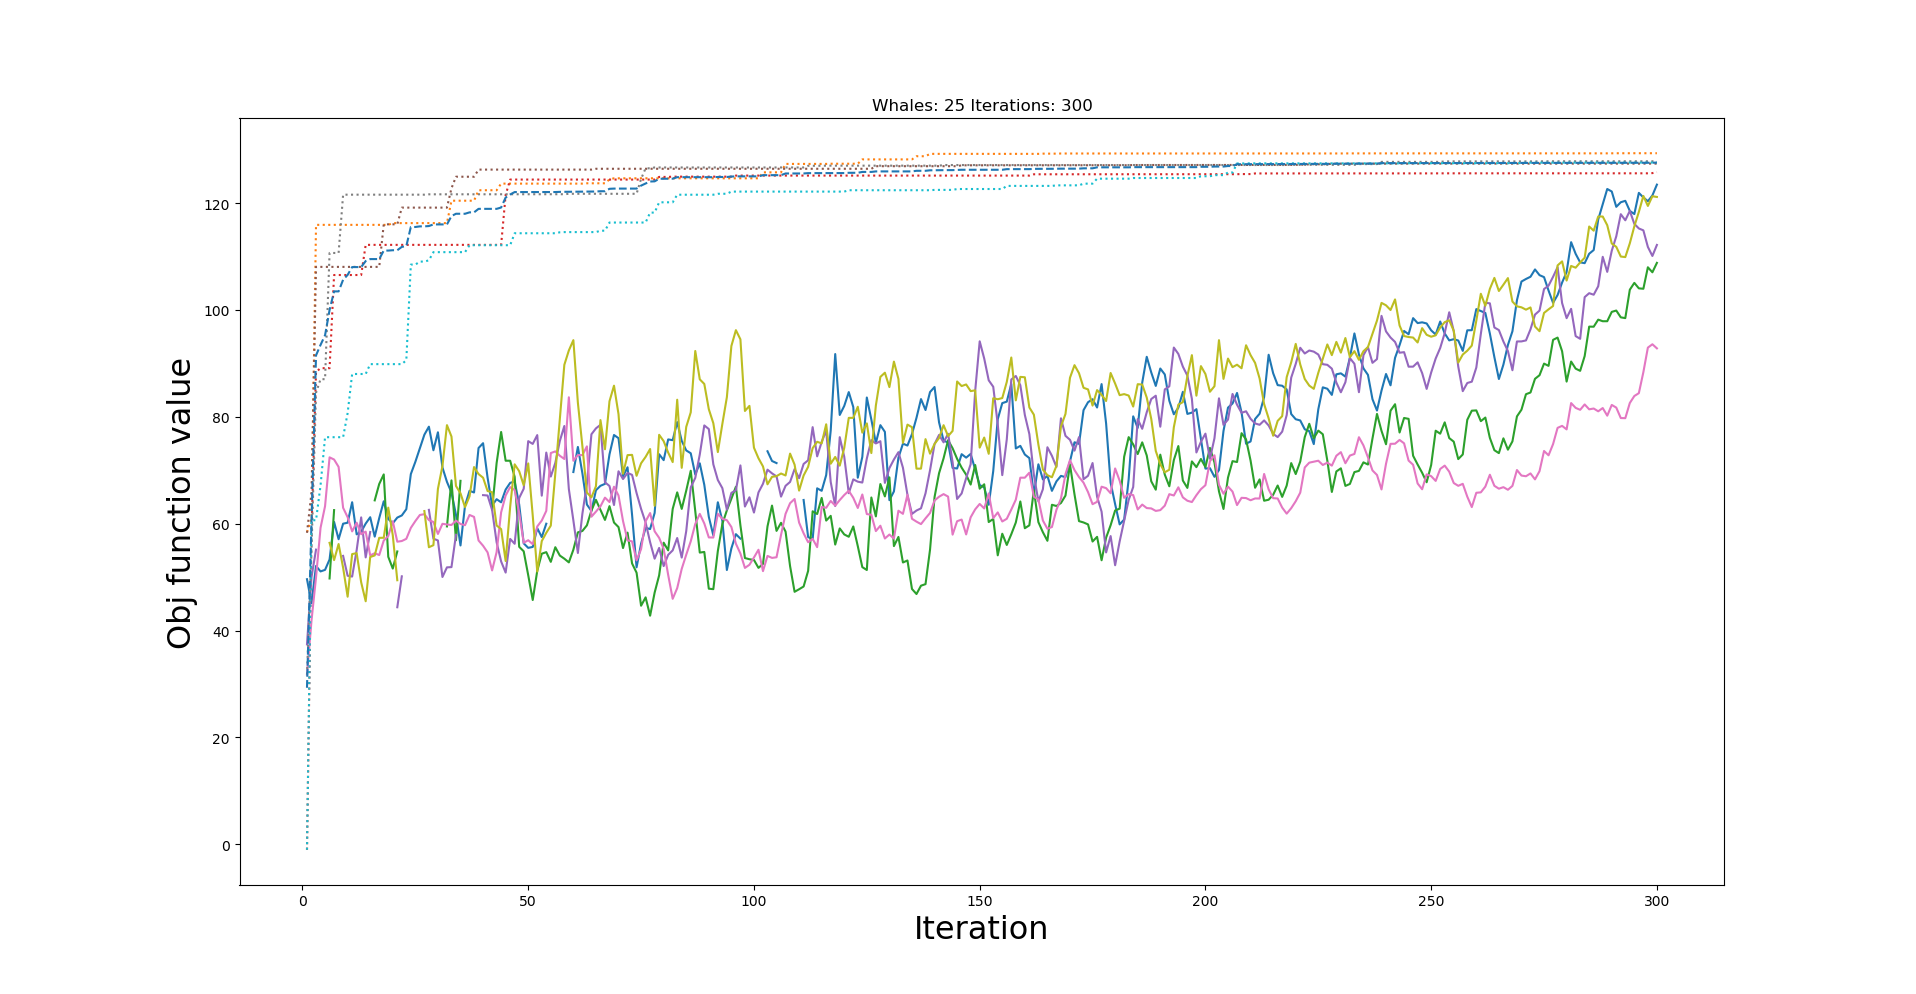
\includegraphics[width=1\linewidth]{Figure_4}
		\caption{Objective function trends for peg hole task with 25 whales particles for 300 iterations}\label{fig:sfig3}
\end{figure}

In figures \ref{fig:sfig4} and \ref{fig:sfig5} are shown 2 of outputted result configuration, where the Robot 1 is shown fixed at the first point of the trajectory to perform, the external environment is hidden for sake of visualization simplicity.
Figures \ref{fig:sfig6} and \ref{fig:sfig7} show the resulted path solution for a hole peg and trimming operation, where it is noticeable that the path frames exploit the task redundancy by changing the directions along the path.
\begin{figure}[h]
		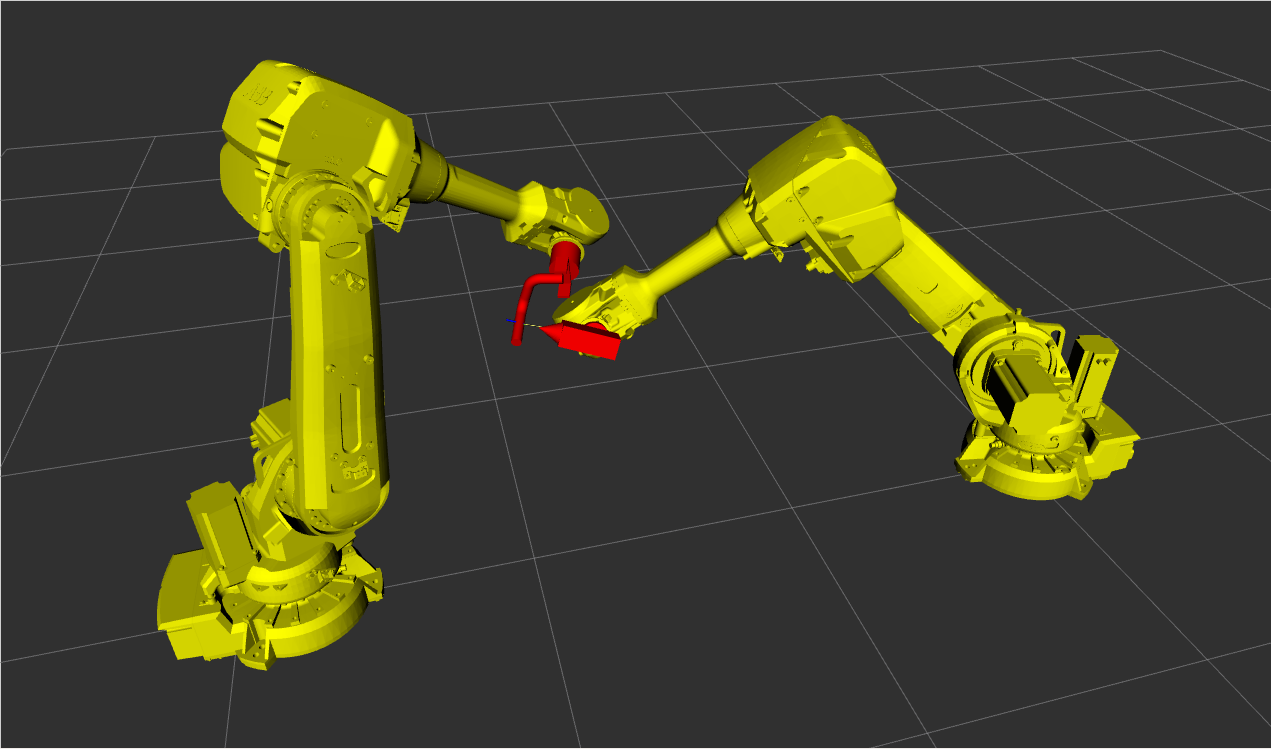
\includegraphics[width=0.9\linewidth]{pos1}
		\caption{cell configuration 1 - peg hole task}
		\label{fig:sfig4}
		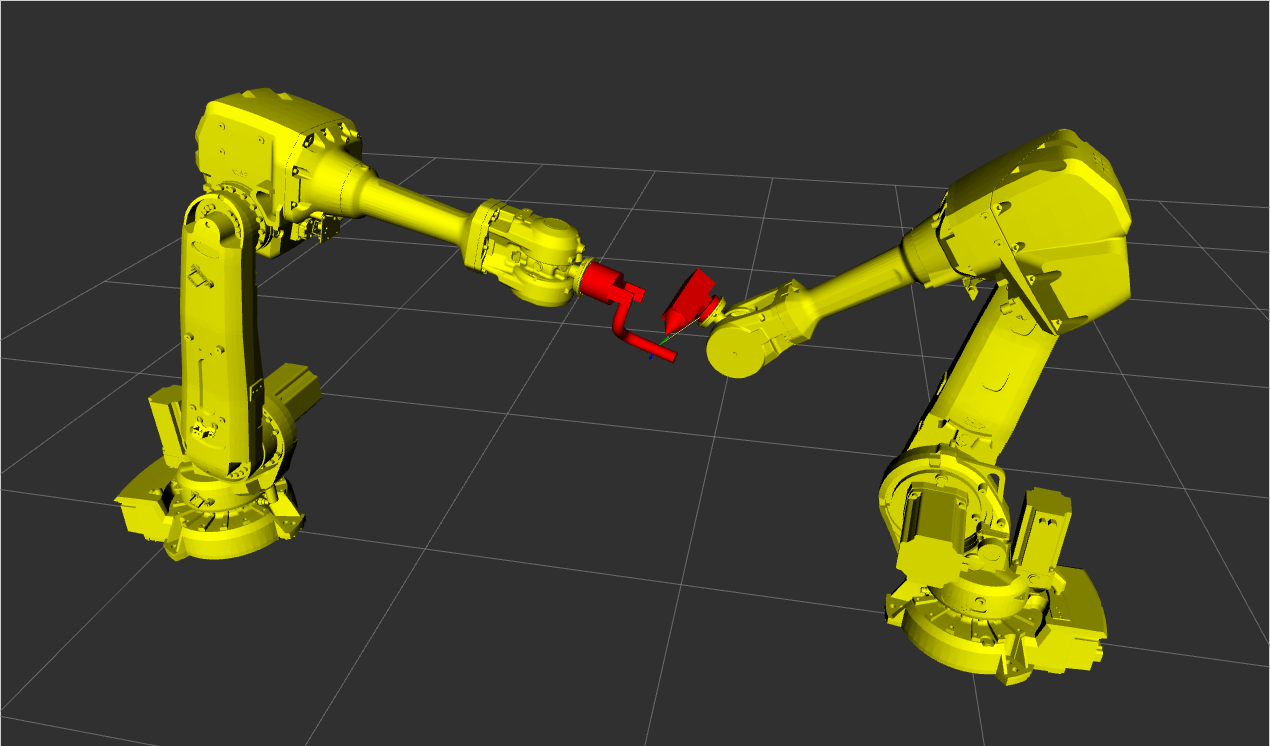
\includegraphics[width=0.9\linewidth]{pos2}
		\caption{cell configuration 2 - tip trimming task}
		\label{fig:sfig5}
\end{figure}

\begin{figure}[h]
		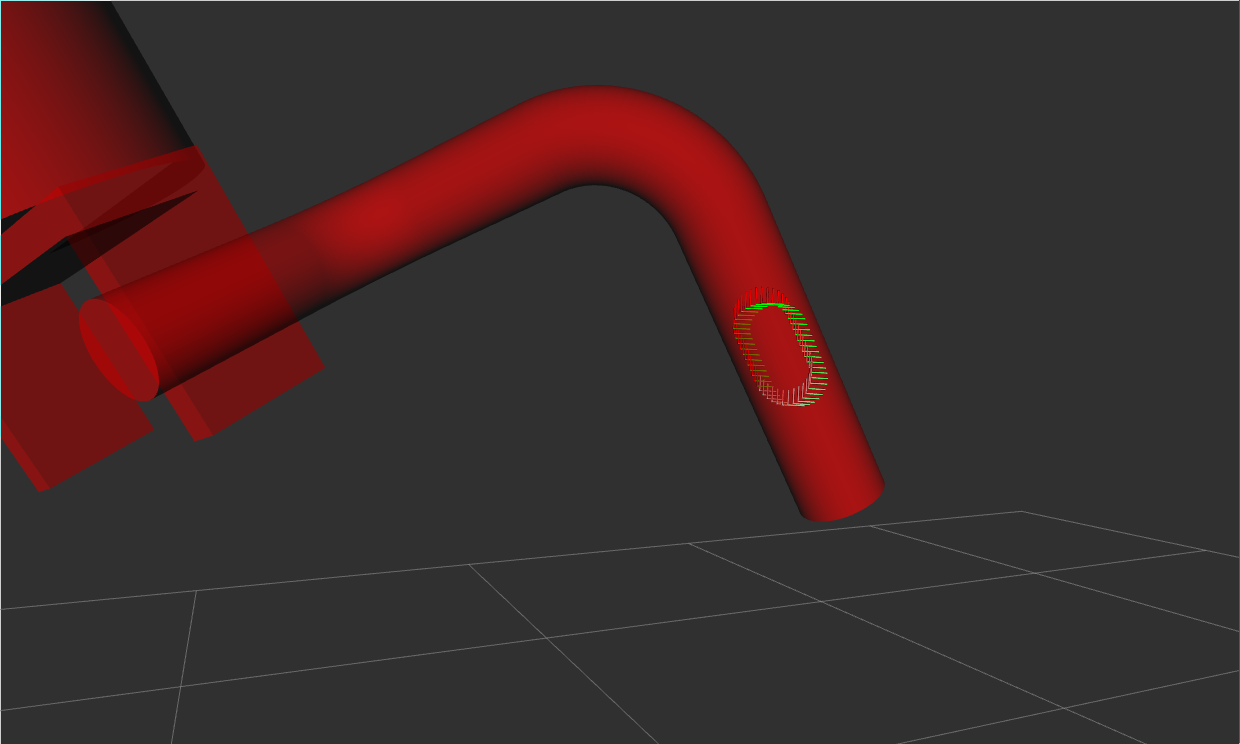
\includegraphics[width=0.8\linewidth]{scr1}
		\caption{path peg hole}
		\label{fig:sfig6}
		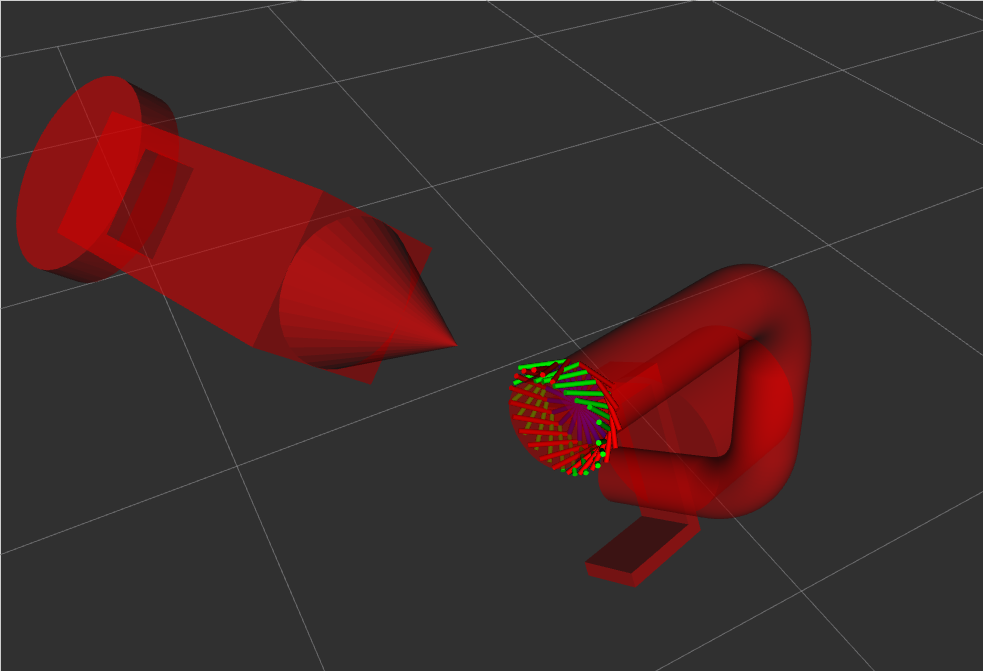
\includegraphics[width=0.8\linewidth]{scr2}
		\caption{path trimming}
		\label{fig:sfig7}
\end{figure}

Furthermore, the algorithm is shown to hugely exploit the available redundancy, changing the TCP orientation during the movement in order to decrease joint speeds and accelerations during the work head re-orien\-tations. 
This increases in cases like the tip trimming, where taking advantage of the task redundancy is crucial to have smooth solutions.
In figure \ref{fig:sfig8}, is shown the average deviation from the nominal $Z$ TCP angle during 2 different types of tasks, collected using 100 experiments per type of task.


\begin{figure}[h]
		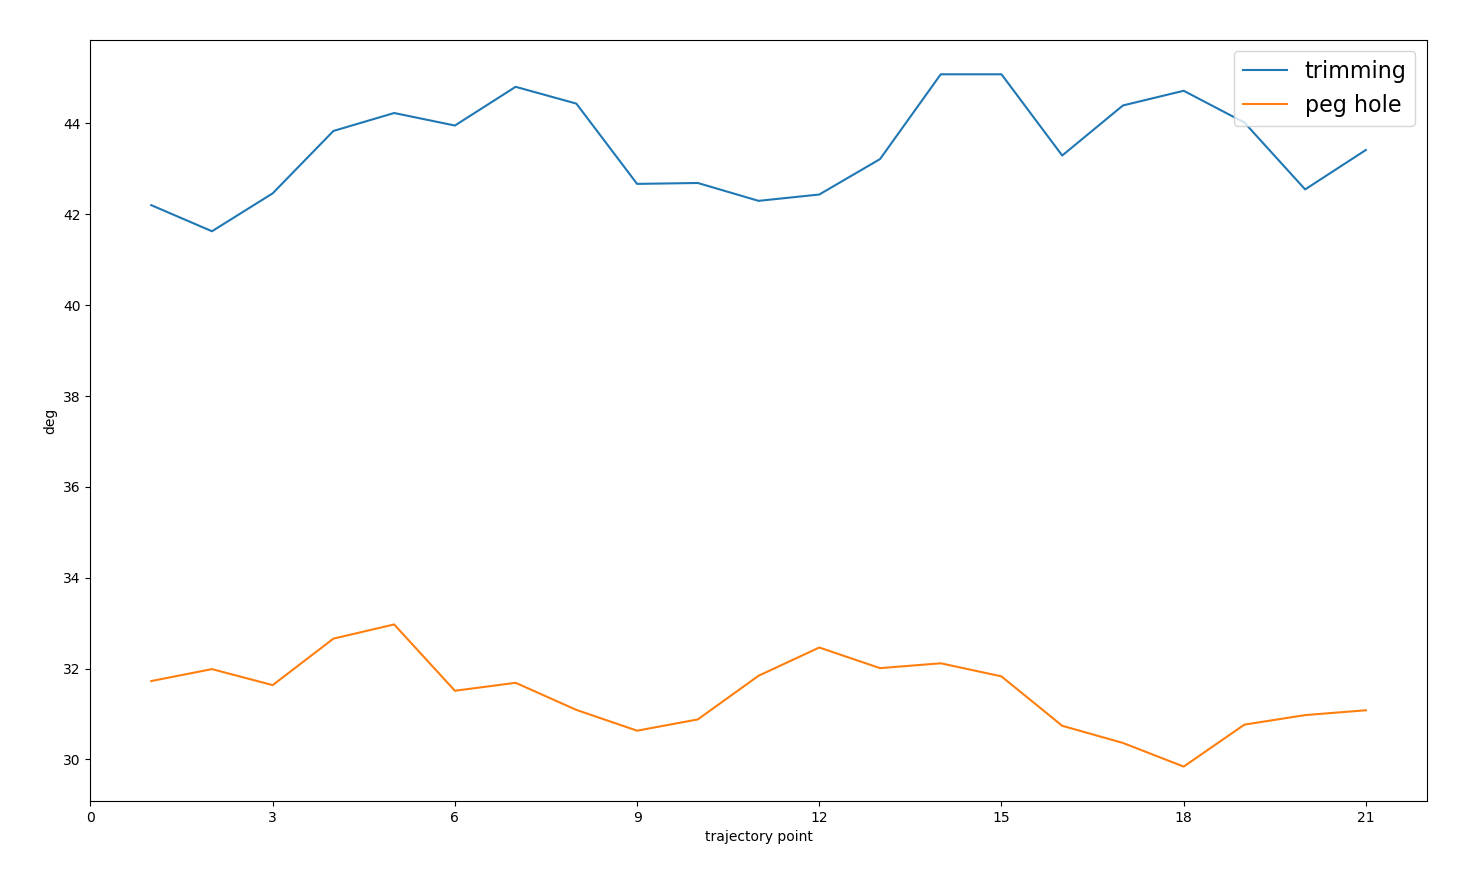
\includegraphics[width=1\linewidth]{red}
		\caption{average redundant angle deviation in degrees from the $Z$ Frenet frame axis, for different tasks, using different WOA parameters, normalized on a 21 point path}
		\label{fig:sfig8}
\end{figure}

\subsection{Parameters influence}
While the internal parameters of the WOA and ACO algorithm have been tuned following state of the art works on the subject, the WACO algorithm presents parameters regarding the number of particles in the WOA algorithm and the corresponding number of iterations.
Namely, the $a_lim$ parameter of the WOA algorithm is set to 1, while the $\beta$ value of the ACO algorithm is set to 2.
The algorithm running time is shown to depend linearly on the number of whales particle and iteration number , as shown in figure \ref{fig:sfig9}, where the average time and its standard deviation are plotted for different parameters.
The running time deviation value is due to the collision checking phase, which is the non-deterministic part of the algorithm in terms of execution time.
The bottom part of figure \ref{fig:sfig9} shows the trend of the objective function value per whales and whales iteration numbers, showing that it has an asymptotic behaviour. 
This behaviour highlights the fact that the optimization problem is well solved with a limited amount of resources and that the solution space is explored adequately.
Figure \ref{fig:sfig10} shows the relations between the objective function value and the computation time, suggesting the parameters zone with a good trade off in term of computation time and result optimality.  
\begin{figure}[h]
		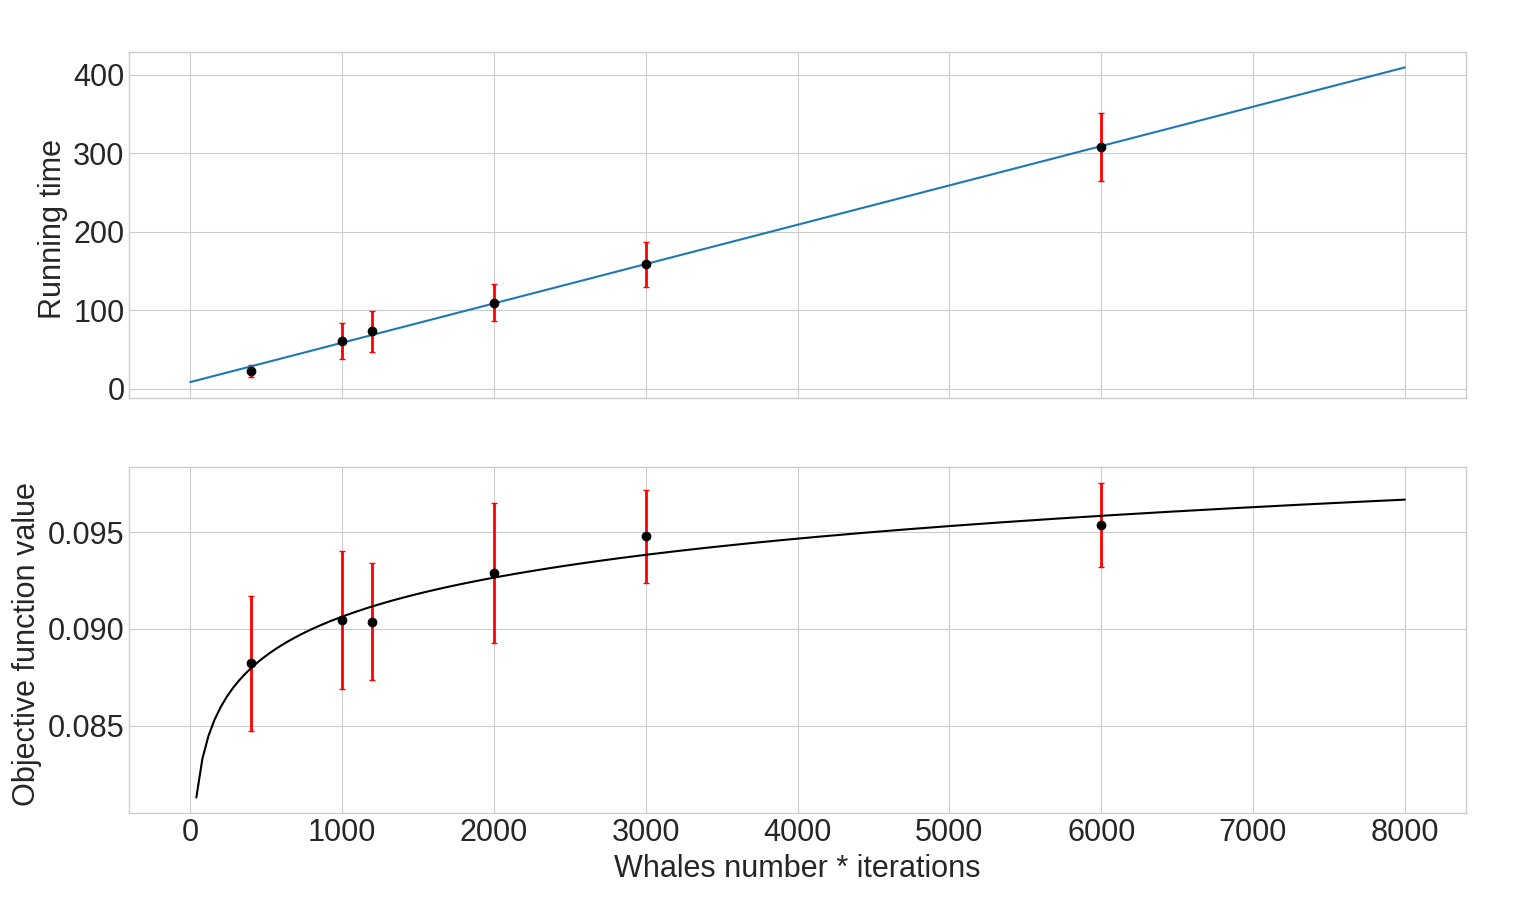
\includegraphics[width=1\linewidth]{solstimes.png}
		\caption{algorithm running time(top) and objective function value(bottom), using number of WOA particles times number of iteration on the abscissa.Fixed number of ACO cycles(50),tip trimming task.Upper figure shows data with a  linear fitting, while the bottom one a natural logarithmic fitting}
		\label{fig:sfig9}
\end{figure}

\begin{figure}[h]
		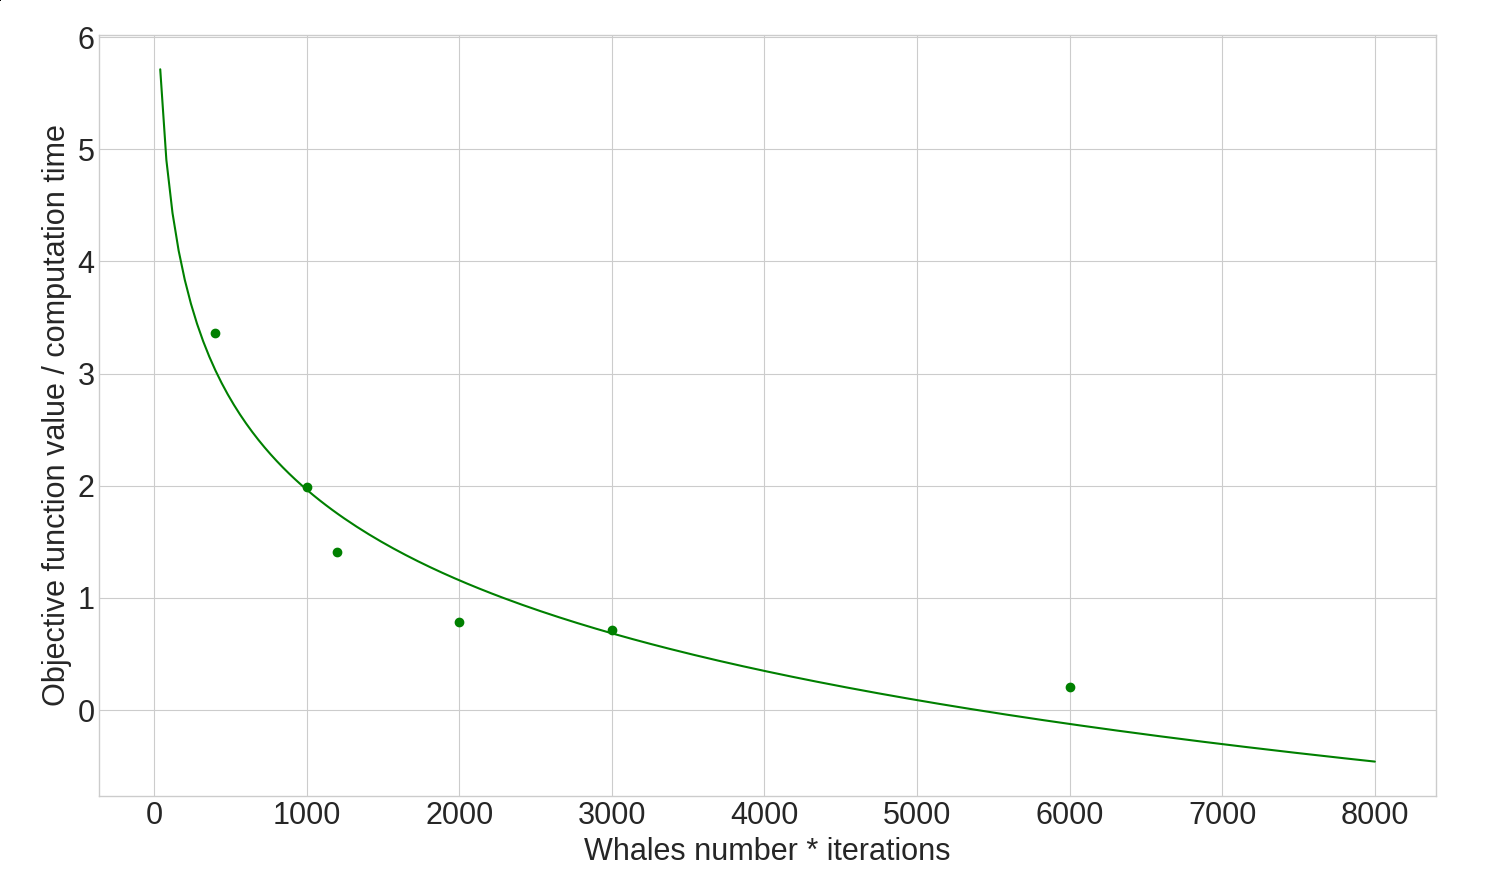
\includegraphics[width=1\linewidth]{objtime.png}
		\caption{ objective function value over algorithm running time, test case same as Figure \ref{fig:sfig9}, data fitted with a natural logarithm }
		\label{fig:sfig10}
\end{figure}

\rev{video?}\\
\rev{ è anche possibile calcolare se conviene come costo computazionale fare l'euristica online o offline, ma non so se lo metterei visto che qua tutto è offline (equazioni sotto).}\\

It is also possible to determine a priori whether is more convenient for the computation time use the offline heuristic and the online heuristic, by computing the number of times a single heuristic value is computed. In case of the offline heuristic it is equal to:
\begin{equation}
    N_{off} = (N_A * N_C)^2 * N_p
\end{equation}
Instead for the online heuristic it is:
\begin{equation}
    N_{onl} = N_{ants}*ACO_{iter}*N_A * N_C *N_p
\end{equation}
So we can define the following ratio $r$ that tells which one is more convenient between online and offline heuristic.
\begin{equation}
r = \frac{N_{off}}{N_{onl}} = \frac{N_A * N_C}{N_{ants}*ACO_{iter}}
\end{equation}
\begin{equation}
\begin{cases}
\text{online heuristic}, & \text{if }r>1   \\
\text{offline heuristic}, & \text{if } r<1
\end{cases}
\end{equation}
\section{Conclusions and future developments}
\label{conclusions}

In this paper a method named WACO (Whale and Ant Colony Optimisation) to optimise task placement for process planning of redundant multi-robot cells is presented, the optimisation is performed by 2 nested meta-heuristic algorithms (WOA and ACO) in order to enhance the overall accuracy of the task. The method assures the kinematic feasibility of the task trajectory and the optimization of collision free trajectories. The WACO has proven to converge to an optimal solution but the calculation time is still not completely satisfying, due to the high amount of offline data to compute. Although, the method is highly parallelizable so the calculation time is expected to decrease.
Future methods improvements might involve the use of online statistical tools to avoid offline computation of graph heuristic values, in order to have a better management of the hardware resources used to run the algorithm.

\rev{aggiungerei che faremo degli sgami per ridurre il consumo di memoria, uno sgamo che avevo pensato ma non mi sono mai sognato di implementare era creare una specie di cache dell'euristica per quando veniva calcolata online}

\begin{acknowledgements}
Evolaser
\end{acknowledgements}

\bibliographystyle{spphys}
\bibliography{biblio}



%\appendix 
%\section{WOA Whale Optimization Algorithm}
%\label{WOA}
%
%In this section, the Whale Optimization Algorithm (WOA) is briefly presented. For a deeper analysis refers to~\cite{Mirjalili2016}.\\
%The algorithms, compared to other well established meta-heuristics algorithms, e.g. the PSO (particle Swarm Optimization), is very competitive~\cite{Mirjalili2016}. It is able to solve a wide range of optimization problems such as uni-modal and multi-modal or with a high number of variables. Moreover, the algorithms allows the user set the ratio between exploration and exploitation. The WOA is a swarm meta-heuristic algorithm that takes inspiration from the hunting strategy of the humpback whales, so 3 heuristics have been developed: the encirclement, the bubble-net attacking method and the exploration.
%
%
%At each iteration the algorithm chooses between the heuristics by means of two coefficients $A$ and $p$. $A$ absolute value decreases linearly from 2 to 0, as the WOA iterations reaches the maximum, meanwhile is modified by a random component, instead $p$ is a random number in $[0,1]$. So the heuristic is chosen as: $p<0.5$ and $|A|<A_{lim}$ Encirclement; $p\geq0.5$ Bubble-net attacking method; $p<0.5$ and $|A|\geq A_{lim}$ Exploration.
%
%The \vv{Encirclement} heuristic mimics the encirclement of the prey so all the whales will position inside an hypercube, the number of dimensions of the hypercube are the number of variables to optimize, whose side is at maximum the distance between the whales and the best so far solution. Moreover as the iterations increases the hypercube will shrink.\\
%The \vv{Bubble-net attacking method} consists in an helix shrinking shaped movement around the prey so the whales will be positioned on a logarithmic spiral centered on the best so far solution, the size of the spiral tends to decrease as the algorithm reaches the maximum iterations.\\
%The \vv{Exploration} is performed similarly to the \vv{Encirclement}, although the hypercube instead of being centered on the best so far solution, is centered on a random chosen whale.
%\begin{algorithm}[t]
%	\scriptsize 
%	\caption{WOA}\label{alg_WOA}
%	\begin{algorithmic}[1]
%		\State Initialize whales positions
%		\State Calculate fitness of every whale
%		\While{$t<max$ $iteration$}
%		\For{each whale}
%		\State Update algorithm parameters
%		\If {$p<0.5$} 
%		\If {$|A|<A_{lim}$}
%		\State Encirclement
%		\Else
%		\State Exploration
%		\EndIf
%		\Else 
%		\State Bubble-net attacking method
%		\EndIf 
%		\EndFor
%		\State Check if any whale is beyond the search space and correct it
%		\State Calculate whales fitness
%		\State Update fittest whale
%		\State $t=t+1$
%		\EndWhile 
%	\end{algorithmic}
%\end{algorithm}
%\\
%The pseudo code of the WOA is in Alg.~\ref{alg_WOA}. The algorithm uses only two heuristics at the same moment. Essentially it depends on $A_{lim}$ and the iteration reached by the algorithm. In the firsts iterations $|A|\geq A_{lim}$ and the algorithm is more focused on the exploration of the search domain, while as it reaches the maximum number of iterations $|A|<A_{lim}$ it optimizes the best solution found. It is possible to set the amount of iterations spent exploring by setting the value of $A_{lim}$.\vspace{-6pt}
%
%\section{ACO Ant Colony Optimization}
%\label{ACO_a}
%
%Ant Colony Optimization (ACO) is a family of well established swarm meta-heuristic algorithms for graph research. In particular, each ant deposes a certain amount of pheromone along its path, so that the following ants will be likely to follow the same path. The pheromone has an evaporation rate, so if the path is not efficient, the pheromone will completely vanish and the following ants will try a different path. There are many variants of the ACO~\cite{Dorigo2006}. In this application it has been used the Ant System as described in \cite{Dorigo1996}.
%
%\begin{algorithm}[t]
%	\caption{ACO}\label{alg_ACO}
%	\scriptsize 
%	\begin{algorithmic}[1]
%		\State Initialize pheromone on the graph
%		\While {$t<max~iterations$}
%		\For{each ant}
%		\For {each graph layer}
%		\State Choose next path node with~(\ref{eq_ACO_path})
%		\EndFor
%		\State Calculate cost on path
%		\EndFor
%		\State Depose pheromone on the graph
%		\State $t=t+1$
%		\EndWhile
%	\end{algorithmic}
%\end{algorithm}
%At each iteration, each ant chooses a path from the starting point to the goal point along a graph, and the ants can move only from one layer to the next one. The path is chosen by combining an heuristic, the pheromone deposited on the graph and a casual component:
%\begin{equation}\vspace{-3pt}
%\small
%\label{eq_ACO_path}
%\begin{aligned}
%&P = heuristic\cdot pheromon	\\ 
%&P_{norm} = \frac{P}{\sum P}	\\ 
%&node= find\biggl(rand[0,1]\leq sum~cum\bigl(P_{norm}\bigr),closest\biggr)
%\end{aligned}
%\end{equation}
%The pheromone deposition is performed at the end of every iteration and is inverse-proportional to a cost function. In Algorithm~\ref{alg_ACO} is shown the pseudo-code of the ACO implemented.

\end{document}

